% Options for packages loaded elsewhere
\PassOptionsToPackage{unicode}{hyperref}
\PassOptionsToPackage{hyphens}{url}
%
\documentclass[
]{book}
\usepackage{amsmath,amssymb}
\usepackage{lmodern}
\usepackage{iftex}
\ifPDFTeX
  \usepackage[T1]{fontenc}
  \usepackage[utf8]{inputenc}
  \usepackage{textcomp} % provide euro and other symbols
\else % if luatex or xetex
  \usepackage{unicode-math}
  \defaultfontfeatures{Scale=MatchLowercase}
  \defaultfontfeatures[\rmfamily]{Ligatures=TeX,Scale=1}
\fi
% Use upquote if available, for straight quotes in verbatim environments
\IfFileExists{upquote.sty}{\usepackage{upquote}}{}
\IfFileExists{microtype.sty}{% use microtype if available
  \usepackage[]{microtype}
  \UseMicrotypeSet[protrusion]{basicmath} % disable protrusion for tt fonts
}{}
\makeatletter
\@ifundefined{KOMAClassName}{% if non-KOMA class
  \IfFileExists{parskip.sty}{%
    \usepackage{parskip}
  }{% else
    \setlength{\parindent}{0pt}
    \setlength{\parskip}{6pt plus 2pt minus 1pt}}
}{% if KOMA class
  \KOMAoptions{parskip=half}}
\makeatother
\usepackage{xcolor}
\usepackage{color}
\usepackage{fancyvrb}
\newcommand{\VerbBar}{|}
\newcommand{\VERB}{\Verb[commandchars=\\\{\}]}
\DefineVerbatimEnvironment{Highlighting}{Verbatim}{commandchars=\\\{\}}
% Add ',fontsize=\small' for more characters per line
\usepackage{framed}
\definecolor{shadecolor}{RGB}{248,248,248}
\newenvironment{Shaded}{\begin{snugshade}}{\end{snugshade}}
\newcommand{\AlertTok}[1]{\textcolor[rgb]{0.94,0.16,0.16}{#1}}
\newcommand{\AnnotationTok}[1]{\textcolor[rgb]{0.56,0.35,0.01}{\textbf{\textit{#1}}}}
\newcommand{\AttributeTok}[1]{\textcolor[rgb]{0.77,0.63,0.00}{#1}}
\newcommand{\BaseNTok}[1]{\textcolor[rgb]{0.00,0.00,0.81}{#1}}
\newcommand{\BuiltInTok}[1]{#1}
\newcommand{\CharTok}[1]{\textcolor[rgb]{0.31,0.60,0.02}{#1}}
\newcommand{\CommentTok}[1]{\textcolor[rgb]{0.56,0.35,0.01}{\textit{#1}}}
\newcommand{\CommentVarTok}[1]{\textcolor[rgb]{0.56,0.35,0.01}{\textbf{\textit{#1}}}}
\newcommand{\ConstantTok}[1]{\textcolor[rgb]{0.00,0.00,0.00}{#1}}
\newcommand{\ControlFlowTok}[1]{\textcolor[rgb]{0.13,0.29,0.53}{\textbf{#1}}}
\newcommand{\DataTypeTok}[1]{\textcolor[rgb]{0.13,0.29,0.53}{#1}}
\newcommand{\DecValTok}[1]{\textcolor[rgb]{0.00,0.00,0.81}{#1}}
\newcommand{\DocumentationTok}[1]{\textcolor[rgb]{0.56,0.35,0.01}{\textbf{\textit{#1}}}}
\newcommand{\ErrorTok}[1]{\textcolor[rgb]{0.64,0.00,0.00}{\textbf{#1}}}
\newcommand{\ExtensionTok}[1]{#1}
\newcommand{\FloatTok}[1]{\textcolor[rgb]{0.00,0.00,0.81}{#1}}
\newcommand{\FunctionTok}[1]{\textcolor[rgb]{0.00,0.00,0.00}{#1}}
\newcommand{\ImportTok}[1]{#1}
\newcommand{\InformationTok}[1]{\textcolor[rgb]{0.56,0.35,0.01}{\textbf{\textit{#1}}}}
\newcommand{\KeywordTok}[1]{\textcolor[rgb]{0.13,0.29,0.53}{\textbf{#1}}}
\newcommand{\NormalTok}[1]{#1}
\newcommand{\OperatorTok}[1]{\textcolor[rgb]{0.81,0.36,0.00}{\textbf{#1}}}
\newcommand{\OtherTok}[1]{\textcolor[rgb]{0.56,0.35,0.01}{#1}}
\newcommand{\PreprocessorTok}[1]{\textcolor[rgb]{0.56,0.35,0.01}{\textit{#1}}}
\newcommand{\RegionMarkerTok}[1]{#1}
\newcommand{\SpecialCharTok}[1]{\textcolor[rgb]{0.00,0.00,0.00}{#1}}
\newcommand{\SpecialStringTok}[1]{\textcolor[rgb]{0.31,0.60,0.02}{#1}}
\newcommand{\StringTok}[1]{\textcolor[rgb]{0.31,0.60,0.02}{#1}}
\newcommand{\VariableTok}[1]{\textcolor[rgb]{0.00,0.00,0.00}{#1}}
\newcommand{\VerbatimStringTok}[1]{\textcolor[rgb]{0.31,0.60,0.02}{#1}}
\newcommand{\WarningTok}[1]{\textcolor[rgb]{0.56,0.35,0.01}{\textbf{\textit{#1}}}}
\usepackage{longtable,booktabs,array}
\usepackage{calc} % for calculating minipage widths
% Correct order of tables after \paragraph or \subparagraph
\usepackage{etoolbox}
\makeatletter
\patchcmd\longtable{\par}{\if@noskipsec\mbox{}\fi\par}{}{}
\makeatother
% Allow footnotes in longtable head/foot
\IfFileExists{footnotehyper.sty}{\usepackage{footnotehyper}}{\usepackage{footnote}}
\makesavenoteenv{longtable}
\usepackage{graphicx}
\makeatletter
\def\maxwidth{\ifdim\Gin@nat@width>\linewidth\linewidth\else\Gin@nat@width\fi}
\def\maxheight{\ifdim\Gin@nat@height>\textheight\textheight\else\Gin@nat@height\fi}
\makeatother
% Scale images if necessary, so that they will not overflow the page
% margins by default, and it is still possible to overwrite the defaults
% using explicit options in \includegraphics[width, height, ...]{}
\setkeys{Gin}{width=\maxwidth,height=\maxheight,keepaspectratio}
% Set default figure placement to htbp
\makeatletter
\def\fps@figure{htbp}
\makeatother
\setlength{\emergencystretch}{3em} % prevent overfull lines
\providecommand{\tightlist}{%
  \setlength{\itemsep}{0pt}\setlength{\parskip}{0pt}}
\setcounter{secnumdepth}{5}
\usepackage{booktabs}
\ifLuaTeX
  \usepackage{selnolig}  % disable illegal ligatures
\fi
\usepackage[]{natbib}
\bibliographystyle{apalike}
\IfFileExists{bookmark.sty}{\usepackage{bookmark}}{\usepackage{hyperref}}
\IfFileExists{xurl.sty}{\usepackage{xurl}}{} % add URL line breaks if available
\urlstyle{same} % disable monospaced font for URLs
\hypersetup{
  pdftitle={MLDS Ethics - Part 1},
  pdfauthor={Zak Varty},
  hidelinks,
  pdfcreator={LaTeX via pandoc}}

\title{MLDS Ethics - Part 1}
\author{Zak Varty}
\date{2022-07-27}

\usepackage{amsthm}
\newtheorem{theorem}{Theorem}[chapter]
\newtheorem{lemma}{Lemma}[chapter]
\newtheorem{corollary}{Corollary}[chapter]
\newtheorem{proposition}{Proposition}[chapter]
\newtheorem{conjecture}{Conjecture}[chapter]
\theoremstyle{definition}
\newtheorem{definition}{Definition}[chapter]
\theoremstyle{definition}
\newtheorem{example}{Example}[chapter]
\theoremstyle{definition}
\newtheorem{exercise}{Exercise}[chapter]
\theoremstyle{definition}
\newtheorem{hypothesis}{Hypothesis}[chapter]
\theoremstyle{remark}
\newtheorem*{remark}{Remark}
\newtheorem*{solution}{Solution}
\begin{document}
\maketitle

{
\setcounter{tocdepth}{1}
\tableofcontents
}
\hypertarget{welcome}{%
\chapter*{Welcome!}\label{welcome}}
\addcontentsline{toc}{chapter}{Welcome!}

Data-driven decision making is now pervasive and impacts us all. Your data is used by others to make decisions about who you are, how you will behave, and what options should be made available to you. Predictive models are used to decide anything from the promotion that is offered to you by a retailer through to whether your loan application is granted by a bank.

The ways in which these predictive models can fail \emph{mathematically} form a core part of the training for an aspiring statistician, data scientist or machine learning practitioner. In contrast, the potential for \emph{ethical} failures in these same models is rarely covered in-depth during as part of this initial training. As a result, these ethical modes of failure are often not considered until those predictive models have been put into production and are actively causing harm.

To prevent this harm, the ethical impacts of using data to make decisions must be made core to the curriculum of both statistics and data science. This course aims to address that gap.

The course takes a practical and technical approach to identifying these ethical issues. It has a strong mathematical focus and will not not require the authoring of extended essays or moral treaties. Throughout the course, we give actionable ways in which these topics may be integrated into a data science workflow at a range of levels.

\hypertarget{module-description}{%
\section*{Module Description}\label{module-description}}
\addcontentsline{toc}{section}{Module Description}

This module will investigate the ethical implications of the new capabilities offered by Data Science and Artificial Intelligence.

Part 1 will begin by discussing the ethical use of data itself - the raw materials of data science pipelines. It will then discuss sets of principles that tech leaders and international bodies are adopting to promote ethical use of data science and artificial intelligence algorithms, including a discussion of real-world examples of failings and adverse outcomes.

Parts 2 and 3 will then revisit the issues explored in Part 1 in greater technical detail. These parts will introduce data science methodologies that provide novel solutions to ethical problems of old such as explainability, prejudice and bias.

\hypertarget{learning-objectives}{%
\section*{Learning Objectives}\label{learning-objectives}}
\addcontentsline{toc}{section}{Learning Objectives}

On successful completion of this module, you should be able to:

\begin{enumerate}
\def\labelenumi{\arabic{enumi}.}
\tightlist
\item
  Recognise and accept responsibility for the societal impact of data science and machine learning technologies;
\item
  Participate in the broader debate about the issues surrounding the use of data science and machine learning for prediction, decision making and knowledge generation tasks;
\item
  Identify common ethical pitfalls of data science and ML algorithms via a mental ``check-list'' and evaluate the degree to which a given algorithm is likely to conform with ethical best practices.
\item
  Formally test for common ethical pitfalls of data science and ML algorithms.
\item
  Implement mitigation measures against the ethical risks posed by the use of data science and ML algorithms.
\item
  Construct well-founded and evidence-based arguments with which to positively influence the actions of stakeholders and decision-makers;
\item
  Use a systems perspective to holistically appraise data science projects on their ethical and societal impacts.
\end{enumerate}

\hypertarget{contributors}{%
\section*{Contributors}\label{contributors}}
\addcontentsline{toc}{section}{Contributors}

These notes are structured around a course delivered as part of the the Master's degree in Machine Learning and Data Science at Imperial College London, which was developed by Christoforos Anagnostopoulos and Zak Varty.

These course notes were written by Zak Varty and are still under active development. If you spot any issues or would like to contribute to their development, you may \href{https://github.com/zakvarty/ethics-1/issues}{raise an issue} or \href{https://github.com/zakvarty/ethics-1/pulls}{submit a pull request} to the associated github repository.

\hypertarget{course-overview}{%
\chapter*{Course Overview}\label{course-overview}}
\addcontentsline{toc}{chapter}{Course Overview}

This section is only relevant to students taking the MLDS course in the academic year 2022-23.

\hypertarget{assessments}{%
\section{Assessments}\label{assessments}}

\begin{longtable}[]{@{}
  >{\raggedright\arraybackslash}p{(\columnwidth - 8\tabcolsep) * \real{0.1250}}
  >{\raggedright\arraybackslash}p{(\columnwidth - 8\tabcolsep) * \real{0.5000}}
  >{\raggedright\arraybackslash}p{(\columnwidth - 8\tabcolsep) * \real{0.1250}}
  >{\raggedright\arraybackslash}p{(\columnwidth - 8\tabcolsep) * \real{0.1250}}
  >{\raggedright\arraybackslash}p{(\columnwidth - 8\tabcolsep) * \real{0.1250}}@{}}
\caption{Assessment schedule for Ethics Part 1 (2022 Cohort)}\tabularnewline
\toprule()
\begin{minipage}[b]{\linewidth}\raggedright
Assessment Type
\end{minipage} & \begin{minipage}[b]{\linewidth}\raggedright
Description
\end{minipage} & \begin{minipage}[b]{\linewidth}\raggedright
\% of Ethics Module
\end{minipage} & \begin{minipage}[b]{\linewidth}\raggedright
Release Date
\end{minipage} & \begin{minipage}[b]{\linewidth}\raggedright
Due Date
\end{minipage} \\
\midrule()
\endfirsthead
\toprule()
\begin{minipage}[b]{\linewidth}\raggedright
Assessment Type
\end{minipage} & \begin{minipage}[b]{\linewidth}\raggedright
Description
\end{minipage} & \begin{minipage}[b]{\linewidth}\raggedright
\% of Ethics Module
\end{minipage} & \begin{minipage}[b]{\linewidth}\raggedright
Release Date
\end{minipage} & \begin{minipage}[b]{\linewidth}\raggedright
Due Date
\end{minipage} \\
\midrule()
\endhead
Reading Summaries & Weekly summary of one assigned reading and peer-feedback for two other students. & 5 & TBC & TBC \\
Coursework & Individual short report. This will involve a mixture of questions and guided case-studies to assess technical understanding of the course content alongside its implementation and limitations when used in context. & 15 & TBC & TBC \\
\bottomrule()
\end{longtable}

\hypertarget{ch-foundations}{%
\chapter{Foundations of Ethical AI}\label{ch-foundations}}

All chapters start with a first-level heading followed by your chapter title, like the line above. There should be only one first-level heading (\texttt{\#}) per .Rmd file.

\hypertarget{a-section}{%
\section{A section}\label{a-section}}

All chapter sections start with a second-level (\texttt{\#\#}) or higher heading followed by your section title, like the sections above and below here. You can have as many as you want within a chapter.

\hypertarget{an-unnumbered-section}{%
\subsection*{An unnumbered section}\label{an-unnumbered-section}}
\addcontentsline{toc}{subsection}{An unnumbered section}

Chapters and sections are numbered by default. To un-number a heading, add a \texttt{\{.unnumbered\}} or the shorter \texttt{\{-\}} at the end of the heading, like in this section.

\hypertarget{ch-privacy-and-autonomy}{%
\chapter{Privacy and Autonomy}\label{ch-privacy-and-autonomy}}

Cross-references make it easier for your readers to find and link to elements in your book.

\hypertarget{captioned-figures-and-tables}{%
\section{Captioned figures and tables}\label{captioned-figures-and-tables}}

Figures and tables \emph{with captions} can also be cross-referenced from elsewhere in your book using \texttt{\textbackslash{}@ref(fig:chunk-label)} and \texttt{\textbackslash{}@ref(tab:chunk-label)}, respectively.

See Figure \ref{fig:nice-fig}.

\begin{Shaded}
\begin{Highlighting}[]
\FunctionTok{par}\NormalTok{(}\AttributeTok{mar =} \FunctionTok{c}\NormalTok{(}\DecValTok{4}\NormalTok{, }\DecValTok{4}\NormalTok{, .}\DecValTok{1}\NormalTok{, .}\DecValTok{1}\NormalTok{))}
\FunctionTok{plot}\NormalTok{(pressure, }\AttributeTok{type =} \StringTok{\textquotesingle{}b\textquotesingle{}}\NormalTok{, }\AttributeTok{pch =} \DecValTok{19}\NormalTok{)}
\end{Highlighting}
\end{Shaded}

\begin{figure}

{\centering 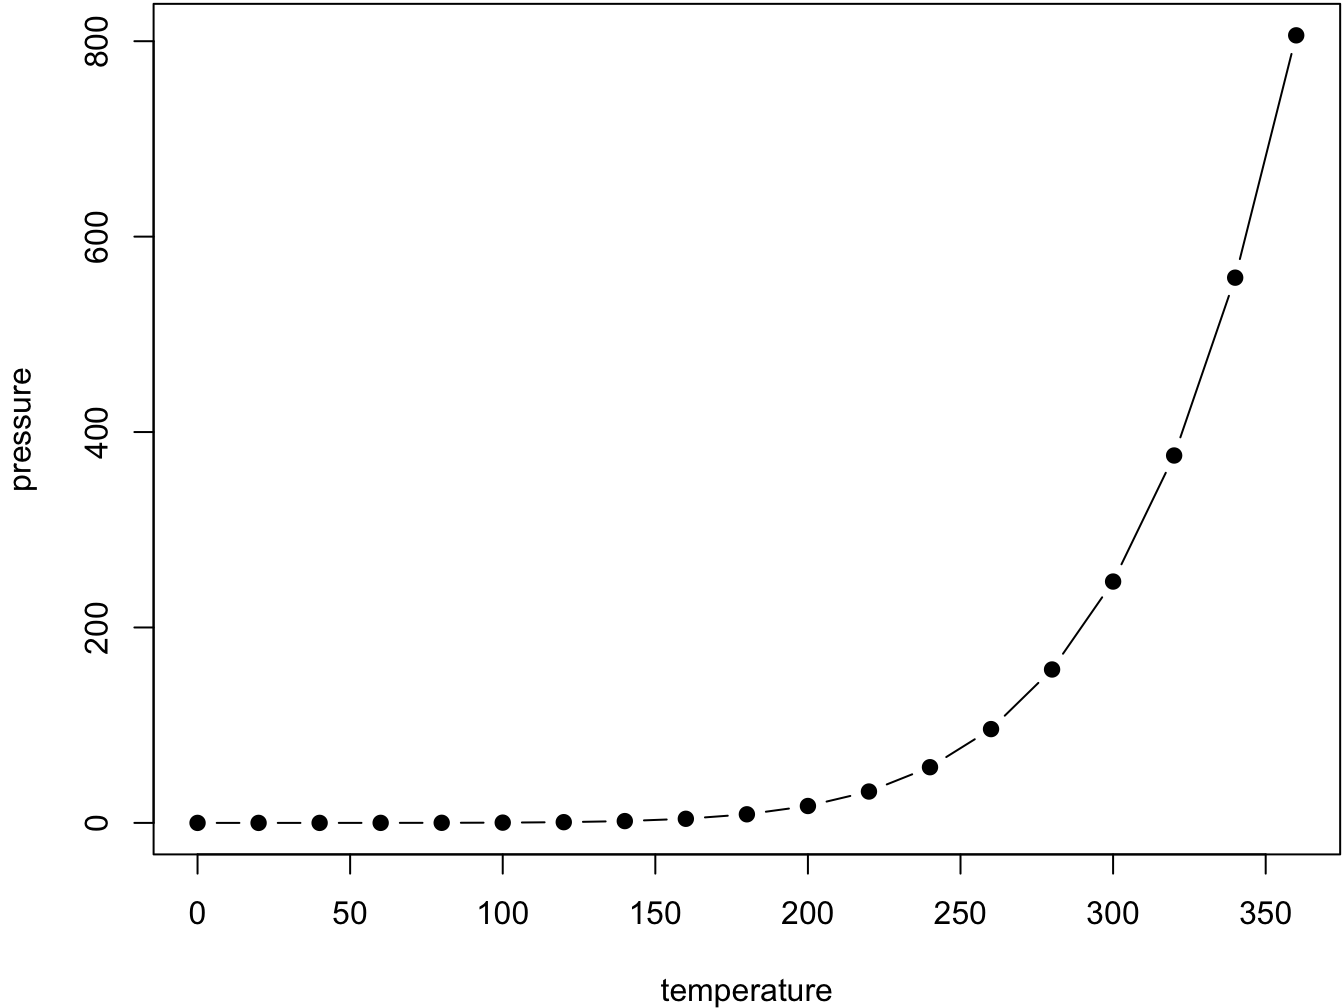
\includegraphics[width=0.8\linewidth]{02-privacy-and-autonomy_files/figure-latex/nice-fig-1} 

}

\caption{Here is a nice figure!}\label{fig:nice-fig}
\end{figure}

Don't miss Table \ref{tab:nice-tab}.

\begin{Shaded}
\begin{Highlighting}[]
\NormalTok{knitr}\SpecialCharTok{::}\FunctionTok{kable}\NormalTok{(}
  \FunctionTok{head}\NormalTok{(pressure, }\DecValTok{10}\NormalTok{), }\AttributeTok{caption =} \StringTok{\textquotesingle{}Here is a nice table!\textquotesingle{}}\NormalTok{,}
  \AttributeTok{booktabs =} \ConstantTok{TRUE}
\NormalTok{)}
\end{Highlighting}
\end{Shaded}

\begin{table}

\caption{\label{tab:nice-tab}Here is a nice table!}
\centering
\begin{tabular}[t]{rr}
\toprule
temperature & pressure\\
\midrule
0 & 0.0002\\
20 & 0.0012\\
40 & 0.0060\\
60 & 0.0300\\
80 & 0.0900\\
\addlinespace
100 & 0.2700\\
120 & 0.7500\\
140 & 1.8500\\
160 & 4.2000\\
180 & 8.8000\\
\bottomrule
\end{tabular}
\end{table}

\hypertarget{ch-fairness}{%
\chapter{Fairness}\label{ch-fairness}}

You can add parts to organize one or more book chapters together. Parts can be inserted at the top of an .Rmd file, before the first-level chapter heading in that same file.

Add a numbered part: \texttt{\#\ (PART)\ Act\ one\ \{-\}} (followed by \texttt{\#\ A\ chapter})

Add an unnumbered part: \texttt{\#\ (PART\textbackslash{}*)\ Act\ one\ \{-\}} (followed by \texttt{\#\ A\ chapter})

Add an appendix as a special kind of un-numbered part: \texttt{\#\ (APPENDIX)\ Other\ stuff\ \{-\}} (followed by \texttt{\#\ A\ chapter}). Chapters in an appendix are prepended with letters instead of numbers.

\hypertarget{ch-alignment-and-control}{%
\chapter{Alignment and Control}\label{ch-alignment-and-control}}

\hypertarget{footnotes}{%
\section{Footnotes}\label{footnotes}}

Footnotes are put inside the square brackets after a caret \texttt{\^{}{[}{]}}. Like this one \footnote{This is a footnote.}.

\hypertarget{citations}{%
\section{Citations}\label{citations}}

Reference items in your bibliography file(s) using \texttt{@key}.

For example, we are using the \textbf{bookdown} package \citep{R-bookdown} (check out the last code chunk in index.Rmd to see how this citation key was added) in this sample book, which was built on top of R Markdown and \textbf{knitr} \citep{xie2015} (this citation was added manually in an external file book.bib).
Note that the \texttt{.bib} files need to be listed in the index.Rmd with the YAML \texttt{bibliography} key.

The \texttt{bs4\_book} theme makes footnotes appear inline when you click on them. In this example book, we added \texttt{csl:\ chicago-fullnote-bibliography.csl} to the \texttt{index.Rmd} YAML, and include the \texttt{.csl} file. To download a new style, we recommend: \url{https://www.zotero.org/styles/}

The RStudio Visual Markdown Editor can also make it easier to insert citations: \url{https://rstudio.github.io/visual-markdown-editing/\#/citations}

\hypertarget{ch-explainability}{%
\chapter{Explainability and Interpretability}\label{ch-explainability}}

\hypertarget{equations}{%
\section{Equations}\label{equations}}

Here is an equation.

\begin{equation} 
  f\left(k\right) = \binom{n}{k} p^k\left(1-p\right)^{n-k}
  \label{eq:binom}
\end{equation}

You may refer to using \texttt{\textbackslash{}@ref(eq:binom)}, like see Equation \eqref{eq:binom}.

\hypertarget{theorems-and-proofs}{%
\section{Theorems and proofs}\label{theorems-and-proofs}}

\begin{theorem}
\protect\hypertarget{thm:tri}{}\label{thm:tri}For a right triangle, if \(c\) denotes the \emph{length} of the hypotenuse
and \(a\) and \(b\) denote the lengths of the \textbf{other} two sides, we have
\[a^2 + b^2 = c^2\]
\end{theorem}

Labeled theorems can be referenced in text using \texttt{\textbackslash{}@ref(thm:tri)}, for example, check out this smart theorem \ref{thm:tri}.

Read more here \url{https://bookdown.org/yihui/bookdown/markdown-extensions-by-bookdown.html}.

\hypertarget{callout-blocks}{%
\section{Callout blocks}\label{callout-blocks}}

The \texttt{bs4\_book} theme also includes special callout blocks, like this \texttt{.rmdnote}.

You can use \textbf{markdown} inside a block.

\begin{Shaded}
\begin{Highlighting}[]
\FunctionTok{head}\NormalTok{(beaver1, }\AttributeTok{n =} \DecValTok{5}\NormalTok{)}
\CommentTok{\#\textgreater{}   day time  temp activ}
\CommentTok{\#\textgreater{} 1 346  840 36.33     0}
\CommentTok{\#\textgreater{} 2 346  850 36.34     0}
\CommentTok{\#\textgreater{} 3 346  900 36.35     0}
\CommentTok{\#\textgreater{} 4 346  910 36.42     0}
\CommentTok{\#\textgreater{} 5 346  920 36.55     0}
\end{Highlighting}
\end{Shaded}

It is up to the user to define the appearance of these blocks for LaTeX output.

You may also use: \texttt{.rmdcaution}, \texttt{.rmdimportant}, \texttt{.rmdtip}, or \texttt{.rmdwarning} as the block name.

The R Markdown Cookbook provides more help on how to use custom blocks to design your own callouts: \url{https://bookdown.org/yihui/rmarkdown-cookbook/custom-blocks.html}

\hypertarget{ch-safety}{%
\chapter{Safety, Security and Accountability}\label{ch-safety}}

\hypertarget{publishing}{%
\section{Publishing}\label{publishing}}

HTML books can be published online, see: \url{https://bookdown.org/yihui/bookdown/publishing.html}

\hypertarget{pages}{%
\section{404 pages}\label{pages}}

By default, users will be directed to a 404 page if they try to access a webpage that cannot be found. If you'd like to customize your 404 page instead of using the default, you may add either a \texttt{\_404.Rmd} or \texttt{\_404.md} file to your project root and use code and/or Markdown syntax.

\hypertarget{metadata-for-sharing}{%
\section{Metadata for sharing}\label{metadata-for-sharing}}

Bookdown HTML books will provide HTML metadata for social sharing on platforms like Twitter, Facebook, and LinkedIn, using information you provide in the \texttt{index.Rmd} YAML. To setup, set the \texttt{url} for your book and the path to your \texttt{cover-image} file. Your book's \texttt{title} and \texttt{description} are also used.

This \texttt{bs4\_book} provides enhanced metadata for social sharing, so that each chapter shared will have a unique description, auto-generated based on the content.

Specify your book's source repository on GitHub as the \texttt{repo} in the \texttt{\_output.yml} file, which allows users to view each chapter's source file or suggest an edit. Read more about the features of this output format here:

\url{https://pkgs.rstudio.com/bookdown/reference/bs4_book.html}

Or use:

\begin{Shaded}
\begin{Highlighting}[]
\NormalTok{?bookdown}\SpecialCharTok{::}\NormalTok{bs4\_book}
\end{Highlighting}
\end{Shaded}

\hypertarget{build-information}{%
\chapter*{Build Information}\label{build-information}}
\addcontentsline{toc}{chapter}{Build Information}

This book was written in \href{http://bookdown.org/}{bookdown} inside \href{http://www.rstudio.com/ide/}{RStudio}. The website \href{https://ethics-1.zakvarty.com}{ethics-1.zakvarty.com} is hosted with \href{https://www.netlify.com}{Netlify}. The complete source is available from \href{https://github.com/zakvarty/ethics-1}{GitHub}.

The \href{assets/ethics-1-logo.png}{course logo} was designed by \href{https://www.zakvarty.com/}{Zak Varty}.

This version of the book was built with:

\begin{verbatim}
#>  setting  value
#>  version  R version 4.2.0 (2022-04-22)
#>  os       macOS Big Sur/Monterey 10.16
#>  system   x86_64, darwin17.0
#>  ui       X11
#>  language (EN)
#>  collate  en_GB.UTF-8
#>  ctype    en_GB.UTF-8
#>  tz       Europe/London
#>  date     2022-07-27
#>  pandoc   2.18 @ /Applications/RStudio.app/Contents/MacOS/quarto/bin/tools/ (via rmarkdown)
\end{verbatim}

Along with these packages:

\begin{tabular}{l|l|l|l}
\hline
Package & Version & Date & Source\\
\hline
bookdown & 0.26 & 2022-04-15 & CRAN (R 4.2.0)\\
\hline
brio & 1.1.3 & 2021-11-30 & CRAN (R 4.2.0)\\
\hline
cachem & 1.0.6 & 2021-08-19 & CRAN (R 4.2.0)\\
\hline
callr & 3.7.0 & 2021-04-20 & CRAN (R 4.2.0)\\
\hline
cli & 3.3.0 & 2022-04-25 & CRAN (R 4.2.0)\\
\hline
crayon & 1.5.1 & 2022-03-26 & CRAN (R 4.2.0)\\
\hline
desc & 1.4.1 & 2022-03-06 & CRAN (R 4.2.0)\\
\hline
devtools & 2.4.3 & 2021-11-30 & CRAN (R 4.2.0)\\
\hline
digest & 0.6.29 & 2021-12-01 & CRAN (R 4.2.0)\\
\hline
ellipsis & 0.3.2 & 2021-04-29 & CRAN (R 4.2.0)\\
\hline
evaluate & 0.15 & 2022-02-18 & CRAN (R 4.2.0)\\
\hline
fastmap & 1.1.0 & 2021-01-25 & CRAN (R 4.2.0)\\
\hline
fs & 1.5.2 & 2021-12-08 & CRAN (R 4.2.0)\\
\hline
glue & 1.6.2 & 2022-02-24 & CRAN (R 4.2.0)\\
\hline
htmltools & 0.5.2 & 2021-08-25 & CRAN (R 4.2.0)\\
\hline
knitr & 1.39 & 2022-04-26 & CRAN (R 4.2.0)\\
\hline
lifecycle & 1.0.1 & 2021-09-24 & CRAN (R 4.2.0)\\
\hline
magrittr & 2.0.3 & 2022-03-30 & CRAN (R 4.2.0)\\
\hline
memoise & 2.0.1 & 2021-11-26 & CRAN (R 4.2.0)\\
\hline
pkgbuild & 1.3.1 & 2021-12-20 & CRAN (R 4.2.0)\\
\hline
pkgload & 1.2.4 & 2021-11-30 & CRAN (R 4.2.0)\\
\hline
prettyunits & 1.1.1 & 2020-01-24 & CRAN (R 4.2.0)\\
\hline
processx & 3.5.3 & 2022-03-25 & CRAN (R 4.2.0)\\
\hline
ps & 1.7.0 & 2022-04-23 & CRAN (R 4.2.0)\\
\hline
purrr & 0.3.4 & 2020-04-17 & CRAN (R 4.2.0)\\
\hline
R6 & 2.5.1 & 2021-08-19 & CRAN (R 4.2.0)\\
\hline
remotes & 2.4.2 & 2021-11-30 & CRAN (R 4.2.0)\\
\hline
rlang & 1.0.2 & 2022-03-04 & CRAN (R 4.2.0)\\
\hline
rmarkdown & 2.14 & 2022-04-25 & CRAN (R 4.2.0)\\
\hline
rprojroot & 2.0.3 & 2022-04-02 & CRAN (R 4.2.0)\\
\hline
rstudioapi & 0.13 & 2020-11-12 & CRAN (R 4.2.0)\\
\hline
sessioninfo & 1.2.2 & 2021-12-06 & CRAN (R 4.2.0)\\
\hline
stringi & 1.7.6 & 2021-11-29 & CRAN (R 4.2.0)\\
\hline
stringr & 1.4.0 & 2019-02-10 & CRAN (R 4.2.0)\\
\hline
testthat & 3.1.4 & 2022-04-26 & CRAN (R 4.2.0)\\
\hline
usethis & 2.1.6 & 2022-05-25 & CRAN (R 4.2.0)\\
\hline
withr & 2.5.0 & 2022-03-03 & CRAN (R 4.2.0)\\
\hline
xfun & 0.31 & 2022-05-10 & CRAN (R 4.2.0)\\
\hline
yaml & 2.3.5 & 2022-02-21 & CRAN (R 4.2.0)\\
\hline
\end{tabular}

  \bibliography{book.bib,packages.bib}

\end{document}
